\documentclass[12pt,a4paper,notitlepage]{report}
    \usepackage{polski}
    \usepackage[T1]{fontenc}
    \usepackage[utf8]{inputenc}
    \usepackage[top=2cm, bottom=2cm, left=3cm, right=3cm]{geometry}
    \usepackage{float}
    \usepackage{listings}
    \usepackage{matlab-prettifier}
    \usepackage{graphicx}
    \graphicspath{ {./images/} }
    \makeatletter
    \newcommand{\linia}{\rule{\linewidth}{0.4mm}}
    \renewcommand{\maketitle}{\begin{titlepage}
        \vspace*{1cm}
        \begin{center}\small
        Politechnika Wrocławska\\
        Wydział Elektroniki\\
        Sprawozdanie z laboratoriów NiDUC2
        \end{center}
        \vspace{3cm}
        \noindent\linia
        \begin{center}
          \LARGE \textsc{\@title}
             \end{center}
         \linia
        \vspace{0.5cm}
        \begin{flushright}
        \begin{minipage}{7cm}
        \textit{\small Autorzy:}\\
        \normalsize \textsc{\@author} \par
        \end{minipage}
        \vspace{5cm}

         {\small wtorek TP, 15:15}\\
            dr inż. Jacek Jarnicki
         \end{flushright}
        \vspace*{\stretch{6}}
        \begin{center}
        \@date
        \end{center}
      \end{titlepage}%
    }
    \makeatother
    \author{Alicja Wróbel, 238894\\
    Justyna Skalska, 225942\\
    Dariusz Tomaszewski, 235565}
    \title{Transmisja w systemie FEC\\
    (Forward Error Correctioin)}
    \begin{document}
    \maketitle
    \tableofcontents
    \chapter{Wstęp}
    \section{Opis FEC}
    FEC, czyli Forward Error Correctioin to technika dodawania nadmiarowych bitów do transmisji informacjicyfrowej. Umożliwia ona detekcję błędów powstałych w wyniku zakłóceń, a także na ich całkowitą lub częściową korekcję. Dzięki jej zastosowaniu nie trzeb korzysać z kanału zwrotnego, aby prosić o ponowne przesłanie uszkodzonych informacji.
    \section{Zastosowania}
    Kodowanie korekcyjne jest wykorzystywane wtedy kiedy retransmisja informacji jest kłopotliwa, kosztowna lub niemożliwa. Przykładem zastosowania może być użycie w warstwie fizycznej oraz warstwie łącza danych, gdzie sprawdzane i poprawiane są błędnie przesłane bity w sieci WAN. Jest to wykorzystywane, aby zapewnić odebranie przez warstwę przez warstwę protokołu aplikacji pakietów wolnych od błędów. Kodowanie jest także używane w transmisji radiowej, gdzie w większości przypadków korekta błędów bitowych może być zaimplementowana za pomocą kodowania FEC. Ma ono dobry czas rzeczywisty i nie wymaga informacji zwrotnej, co jest odpowiednie dla komunikacji bezprzewodowej.
    \section{Typy kodowania FEC}
    W rodzinie kodów FEC istnieje wiele różnych kodów korekcji błędów, które używane są w zależnośći od sytuacji. Oto kilka szeroko wykorzystywanych kodów:
    \begin{itemize}
        \item Reeda-Solomona
        \item Golay'a
        \item potrajanie bitów
        \item Hamminga
        \item BCH (Bose–Chaudhuri–Hocquenghem)
        \item cykliczny kod nadmiarowy
        \item kod splotowy
    \end{itemize}
    \chapter{Cel i założenia projektu}
    Głównym celem projektu było napisanie programu ukazującego poszczególne etapy transmisji w systemie FEC, a także ich działanie.\\
    Symulator systemu miał składać się z fragmentów odpowiedzialnych za:
    \begin{itemize}
        \item generację danych przewidzianych do transmisji
        \item kodowanie wysyłanych danych w nadajniku
        \item zmianę niektórych danych w wyniku zakłóceń w kanale transmisyjnym
        \item dekodowanie odebranych danych w odbiorniku\\
    \end{itemize}
    Analiza statystyczna projektu miała polegać na napisaniu programów rejestrujących i analizujących parametry statystyczne transmisji takie jak:
    \begin{itemize}
        \item obliczanie BER dla różnych parametrów systemu
        \item wyznaczanie rozkładu błędów transmisji w czasie
        \item wyznaczanie parametrów opisujących efektywność transmisji\\
    \end{itemize}
    Symulacja FEC wymagała napisania dwóch programów, z których każdy dostarczał wyniki na temat jednego sposobu kodowania  danych.\\
    Pierwszy program polegał na napisaniu kodera potrajającego każdy bit. Dzięki temu istniało mniejsze ryzyko odebrania niepoprawnej wiadomości po jej odkodowaniu. Polegało ono na ustaleniu czy w ciągu trzech bitów znajduje się więcej 1 lub 0. Dzięki temu, że jest to liczba nieparzysta nie istniała możliwość kiedy system nie był w stanie stwierdzić jaką cyfrę otrzymał. Dzięki temu wiadomość mogła zostać odtworzona pomimo zasymulowanych w kanale zakłóceń. Przekłamania zostały spoodowane losowaniem wartośći z rozkładu Gaussa przy ustalonym prawdopodobieństwie wystąpienia błędu.\\\\
    Kolejne zadanie wymagało napisania kodera oraz dekodera BCH (Bose–Chaudhuri– -Hocquenghem). Zdolność korekcyjna tego kodowanie jest większa niż tego wykorzystanego w pierwszym zadaniu. Zależy ona od wybranych parametrów bitów danych \textit{k} oraz bitów korekcyjnych \textit{n-k}, które przedstawia tablica poniżej \textit{(Rysunek 2.1)}.  Przekłamania zostały spoodowane losowaniem wartośći z rozkładu Gaussa przy ustalonym prawdopodobieństwie wystąpienia błędu.
    \begin{figure}[H]
        \centering       
        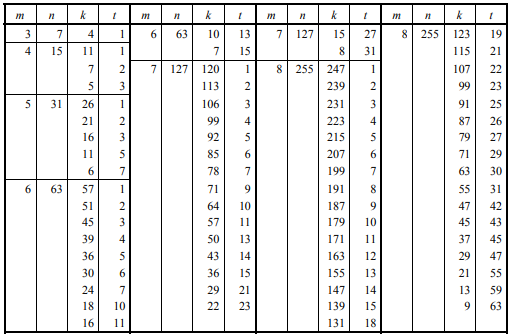
\includegraphics[width=\textwidth]{BCH_table.png}
        \caption{Parametry kodów BCH}
        \label{fig:obrazek BCH_table}
    \end{figure}
    Zadanie projektowe polegało na wykonaniu wielokrotnej symulacji, aby uzyskać pary \textit{(n, k)} wraz z odpowiadającymi im parametrami BER - Bit Error Rate oraz E - Efficency. Prawdopodobieństwo przekłamania jest stałym parametrem, a badane kody BCH odpowiadają n = \{31, 63, 127, 255\}.
    \chapter{Kody źródłowe}
    \section{Potrajanie bitów}
    \subsection{Generator ciągu bitów}
    \lstinputlisting[
        style=Matlab-editor,
        firstline=2,
        basicstyle=\mlttfamily,
        escapechar=`,
        ]{./code/P1/generator.m} \hfill \break
    \subsection{Koder}
    \lstinputlisting[
        style=Matlab-editor,
        firstline=2,
        basicstyle=\mlttfamily,
        escapechar=`,
        ]{./code/P1/koder.m} \hfill \break
    \subsection{Kanał transmisyjny z zakłóceniami}
    \lstinputlisting[
        style=Matlab-editor,
        firstline=2,
        basicstyle=\mlttfamily,
        escapechar=`,
        ]{./code/P1/kanal.m} \hfill \break
    \subsection{Dekoder}
    \lstinputlisting[
        style=Matlab-editor,
        firstline=2,
        basicstyle=\mlttfamily,
        escapechar=`,
        ]{./code/P1/dekoder.m} \hfill \break
    \subsection{BER}
    \lstinputlisting[
        style=Matlab-editor,
        firstline=2,
        basicstyle=\mlttfamily,
        escapechar=`,
        ]{./code/P1/ber.m} \break
    \subsection{Główny kod programu}
    \lstinputlisting[
        style=Matlab-editor,
        firstline=10,
        basicstyle=\mlttfamily,
        escapechar=`,
        ]{./code/P1/main.m} \break
    \section{Kodowanie BCH}
    \subsection{Kanał transmisyjny z zakłóceniami}
    \lstinputlisting[
        style=Matlab-editor,
        firstline=2,
        basicstyle=\mlttfamily,
        escapechar=`,
        ]{./code/P2/kanal.m} \break
    \subsection{Główny kod programu}
    \lstinputlisting[
        style=Matlab-editor,
        firstline=11,
        basicstyle=\mlttfamily,
        escapechar=`,
        ]{./code/P2/main.m} \hfill \break
    \chapter{Wyniki eksperymentu}
    \section{Potrajanie bitów}
    \begin{figure}[H]
        \centering       
        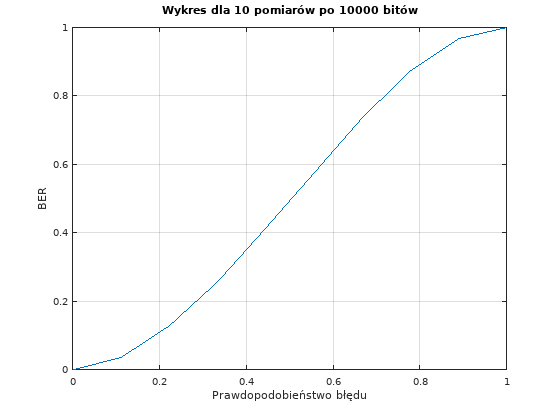
\includegraphics[width=\textwidth]{10_po_10000.png}
        \caption{Liczba błędnie przesłanych pakietów w zależności od prawdopodobieństwa przekłamania w kanale transmisyjnym dla 10 pomiarów po 10000 bitów.}
        \label{fig:obrazek 10_po_10000}
    \end{figure}
    \begin{figure}[H]
        \centering       
        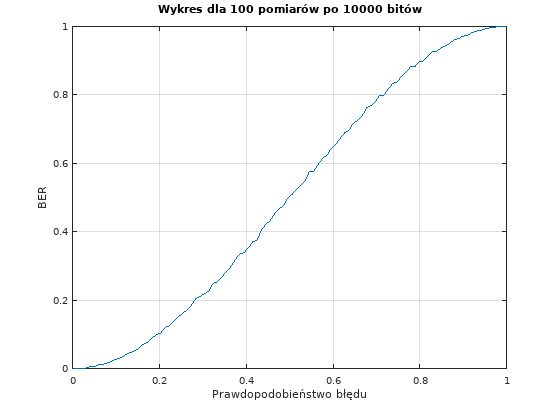
\includegraphics[width=\textwidth]{100_po_10000.png}
        \caption{Liczba błędnie przesłanych pakietów w zależności od prawdopodobieństwa przekłamania w kanale transmisyjnym dla 100 pomiarów po 10000 bitów.}
        \label{fig:obrazek 100_po_10000}
    \end{figure}
    \begin{figure}[H]
        \centering       
        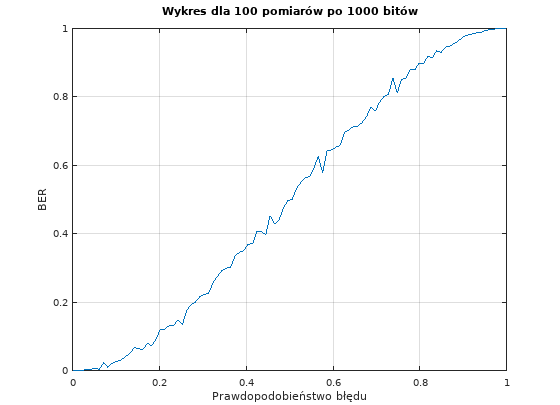
\includegraphics[width=\textwidth]{100_po_1000.png}
        \caption{Liczba błędnie przesłanych pakietów w zależności od prawdopodobieństwa przekłamania w kanale transmisyjnym dla 100 pomiarów po 1000 bitów.}
        \label{fig:obrazek 100_po_1000}
    \end{figure}
    \begin{figure}[H]
        \centering       
        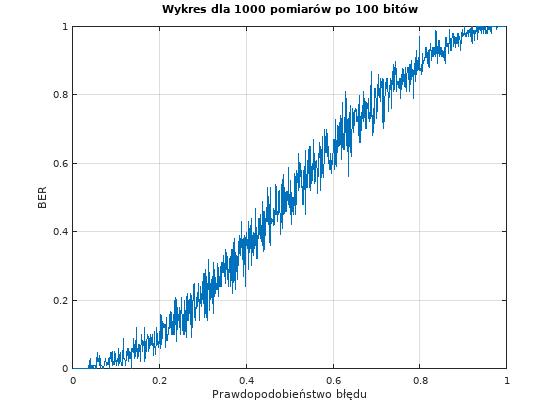
\includegraphics[width=\textwidth]{1000_po_100.png}
        \caption{Liczba błędnie przesłanych pakietów w zależności od prawdopodobieństwa przekłamania w kanale transmisyjnym dla 1000 pomiarów po 100 bitów.}
        \label{fig:obrazek 1000_po_100}
    \end{figure}
    \begin{figure}[H]
        \centering       
        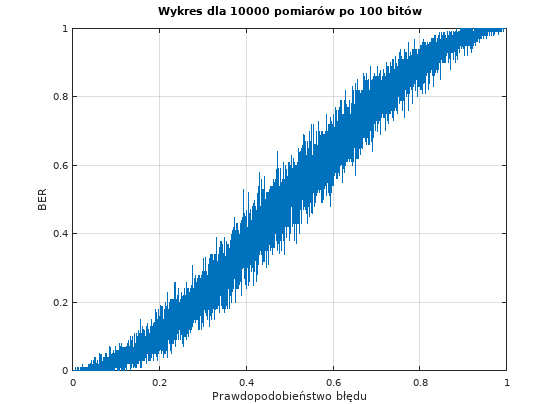
\includegraphics[width=\textwidth]{10000_po_100.png}
        \caption{Liczba błędnie przesłanych pakietów w zależności od prawdopodobieństwa przekłamania w kanale transmisyjnym dla 10000 pomiarów po 100 bitów.}
        \label{fig:obrazek 10000_po_100}
    \end{figure}
    \section{Kodowanie BCH}
    Zadanie projektowe polegało na zasymulowaniu korekcji dla znanych kodów BCH, przy n = \{31, 63, 127, 255\} oraz prawdopodobieństwie przekłamania wynoszącym 0.03. Nie dia się jednoznacznie określić jaki kod BCH jest najbardziej optymalny dla zadanej wartości przekłamania, zaznaczyliśmy, więc na \textit{Rysunek 4.6} najlepsze kody BCH dla naszego kanału transmisyjneg, jest to obszar Pareto.
    \begin{figure}[H]
        \centering       
        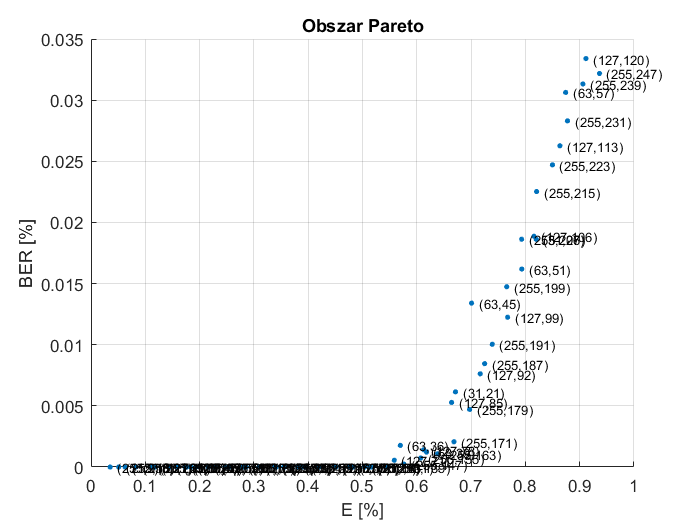
\includegraphics[width=\textwidth]{pareto.png}
        \caption{Obszar Pareto dla prawdopodobieństwa przekłamania = 0.03}
        \label{fig:pareto}
    \end{figure}
    \chapter{Wnioski}
    Bardzo ważnym aspektem przy cyfrowej transmisji danych jest jej niezawodność. Im więcej dobrze odebranych bitów w stosunku do ilości przesłanych tym lepiej. Podczas tworzenia zadania projektowego mogliśmy zobaczyć na czym polega kodowanie i dekodowanie informacji oraz jak duży wpływ na nią może mieć kanał transmisyjny. Dzięki temu wiemy jak ważną rolę przy przesyłaniu danych odgrywa korekcja błędów. Poznaliśmy podstawowe sposoby naprawy źle odebranej informacji.
    \section{Potrajanie bitów}
    Pierwszym zaimplementowanym przez nas kodowaniem było potrajanie bitów. Jest to jeden z najprostszych sposobów kodowania informacji. Jest on jednak mało skuteczny względem innych kodowań, ponieważ korekcja stosunek ilości błędów do ilości przesłanych bitów jest większa niż w pozostałych kodowaniach. Ten elementarny sposób może zostać wykorzystany, gdy wymagania projektu nie oczekują dużej korekcji błędów przesłanej informacji.
    \section{Kodowanie BCH}
    Drugie zaimplementowane przez nas kodowanie cechuje się znacznie większą korekcją błędów w stosunku do poprzednika. Wachlarz zastosowań może być szerszy, ponieważ jesteśmy w stanie poprawić więcej źle odebranych bitów informacji. Kodowanie to wymaga podania parametrów n - długości słowa kodowego oraz k - liczby bitów wiadomości w słowie kodowym. Od nich właśnie zależy zdolność korekcji błędów. Dzięki zadaniu projektowemu mogliśmy nauczyć się jak właściwie zaznaczyć obszar Pareto oraz dzięki temu poprawnie dobrać wartości obu parametrów do wymagań projektowych.
    \begin{thebibliography}{Knuth}
        \addcontentsline{toc}{subsubsection}{Nasz spis publikacji}
        \bibitem{Techopedia} {https://www.techopedia.com/definition/824/forward-error-correction-fec}
        \bibitem{IEEExplore} {https://ieeexplore.ieee.org/document/6201904/}
        \bibitem{MathWorks} {https://www.mathworks.com/help/comm/ref/bchenc.html}
    \end{thebibliography}
\end{document}

% TODO:
%       - zaznaczyć obszar pareto
%       - wnioski
%       opcjonalnie: poprawić kod z 2 etapu  